\documentclass[tikz]{standalone}
\usepackage{fontspec}
\renewcommand*{\familydefault}{\sfdefault}
\usepackage{standalone}
\usepackage{amssymb}
\usetikzlibrary{decorations, shapes.geometric}
%\usetikzlibrary{arrows.meta, decorations.pathmorphing, decorations.pathreplacing, shapes.geometric}
\usetikzlibrary{positioning}
\usetikzlibrary{bayesnet}

\begin{document}
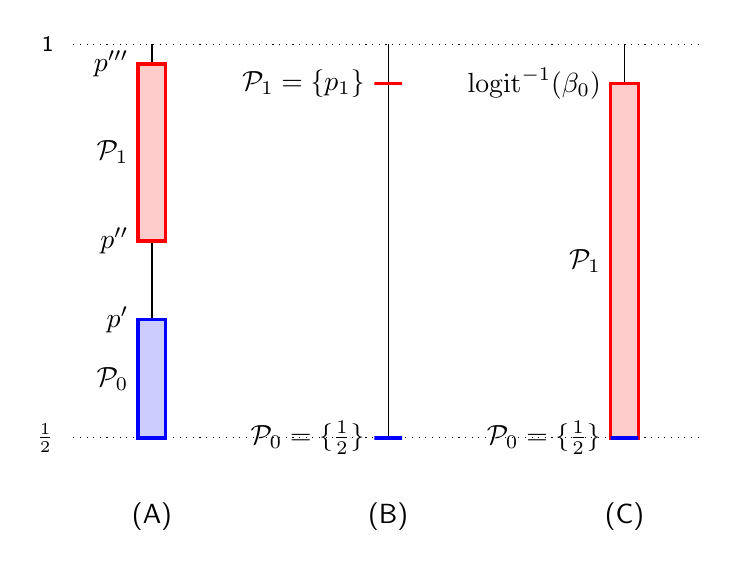
\begin{tikzpicture}%[font=\footnotesize, xscale=1.5]

\draw[dotted, thin, yshift=5 cm] (-1,0) node[label=left:1] (one) {} -- (7,0);
\draw[dotted, thin] (-1,0) node[label=left:\(\frac{1}{2}\)] (half) {} -- (7,0);

\node (a) at (0,-1) {(A)};
\node (b) at (3,-1) {(B)};
\node (c) at (6,-1) {(C)};

\draw
(a|-half) --
node[pos=0.15] (a-P0) {}
node[pos=0.3] (a-P0-r) {}
node[pos=0.5] (a-P1-l) {}
node[pos=0.725] (a-P1) {}
node[pos=0.95] (a-P1-r) {}
(a|-one)
(b|-half) --
node[pos=0] (b-P0-r) {}
node[pos=0.9] (b-P1-l) {}
(b|-one)
(c|-half) --
node[pos=0] (c-P0-r) {}
node[pos=0.45] (c-P1) {}
node[pos=0.9] (c-P1-l) {}
(c|-one)
;

% general
\draw[very thick, red, fill=red!20] ([xshift=-5] a-P1-r) rectangle ([xshift=5] a-P1-l);
\draw[very thick, blue, fill=blue!20] ([xshift=-5] a|-half) rectangle ([xshift=5] a-P0-r);

% M1
\draw[very thick, red, fill=red!20] ([xshift=-5] b-P1-l) rectangle ([xshift=5] b-P1-l);
\draw[very thick, blue, fill=blue!20] ([xshift=-5] b|-half) rectangle ([xshift=5] b-P0-r);

% M2
\draw[very thick, red, fill=red!20] ([xshift=-5] c|-half) rectangle ([xshift=5] c-P1-l);
\draw[very thick, blue, fill=blue!20] ([xshift=-5] c|-half) rectangle ([xshift=5] c-P0-r);

% labels
\begin{scope}[every node/.style={left=5 pt}]
    % (A)
    \node at (a-P0) {\(\mathcal{P}_0\)};
    \node at (a-P0-r) {\(p'\)};
    \node at (a-P1-l) {\(p''\)};
    \node at (a-P1) {\(\mathcal{P}_1\)};
    \node at (a-P1-r) {\(p'''\)};
    % (B)
    \node at (b-P0-r) {\(\mathcal{P}_0=\{\frac{1}{2}\}\)};
    \node at (b-P1-l) {\(\mathcal{P}_1=\{p_1\}\)};
    % (B)
    \node at (c-P0-r) {\(\mathcal{P}_0=\{\frac{1}{2}\}\)};
    \node at (c-P1) {\(\mathcal{P}_1\)};
    \node at (c-P1-l) {\(\mathrm{logit}^{-1}(\beta_0)\)};
\end{scope}

\end{tikzpicture}
\end{document}
